
\section{Algebraic Point Set Surfaces}

The Algebraic Point Set Surfaces \cite{Guennebaud07} method defines an approximate signed distance field from a set of oriented points sampled onto a surface, such that the zero-isosurface best approximates the input points with respect to some given criteria.  It uses local Moving Least Squares (MLS) fitting of algebaic spheres. The implicit function can be evaluated at any point in space with almost no preprocessing.

More specifically, the value of the implicit function $f(x)$ is obtained by fitting an algebraic sphere to the neighbors of the point $x$ in a weighted least square sense where the weights depends on both the Euclidean distance between $x$ and the neighbor points. This weight function behaves like a low pass filter devised to control the degree of smoothing. Intuitively, the fitting algorithm first tries minimizing the distance between the gradient of the algebraic sphere and the input normals, then minimizes the algebraic distance between the 0-isosphere and the neighbors to determine the fitted sphere radius. For these reasons the method is quite sensitive to the quality of the input normals and sampling.

Even though the \ccc{CGAL::APSS_reconstruction_function} class can be used directly, it is aimed to be used with the \cgal\ surface mesh generator to extract its $0$-isosurface.


% Insert image APSS.jpg/eps
\begin{center}
    \label{Surface_reconstruction_points_3-fig-APSS}
    % Image
    \begin{ccTexOnly}
        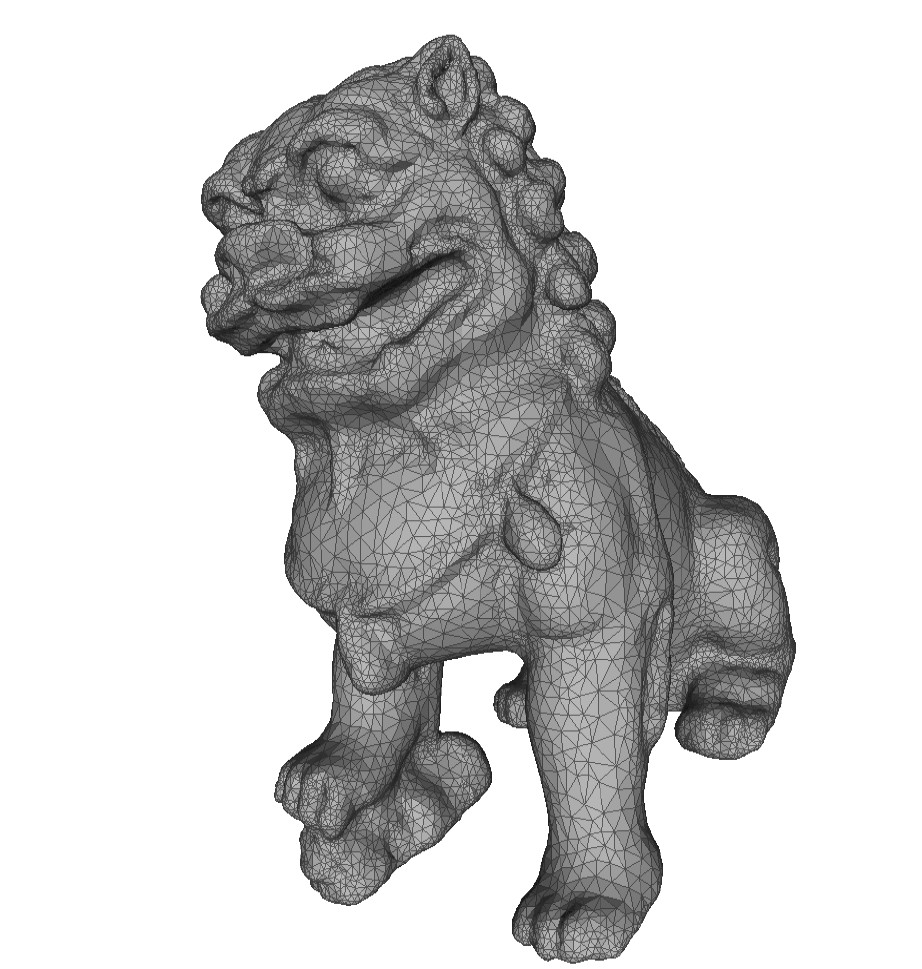
\includegraphics[width=0.5\textwidth]{Surface_reconstruction_points_3/APSS} % omit .eps suffix
    \end{ccTexOnly}
    \begin{ccHtmlOnly}
        <img width="50%" border=0 src="./APSS.jpg"><P>
    \end{ccHtmlOnly}
    % Title
    \begin{figure}[h]
        \caption{APSS surface reconstruction from 10K
                 points sampled with a Minolta laser scanner.}
        % later: add computed function
    \end{figure}
\end{center}

\subsection{Interface}

The class template declaration is:

template$<$  \\
class Gt$>$   \\
class \ccc{APSS_reconstruction_function};

with  \\
\ccc{Gt}: Geometric traits class.


Creation:

% Reduce left margin
\ccTwo{1234567890123456789012}{}

\ccFunction{template<typename InputIterator, typename PointPMap, typename NormalPMap, typename RadiusPMap> APSS_reconstruction_function(InputIterator first, InputIterator beyond, PointPMap point_pmap, NormalPMap normal_pmap, RadiusPMap radius_pmap, FT smoothness);}
{
Creates a APSS implicit function from the [first, beyond) range of points.
\ccCommentHeading{Template Parameters}  \\
\ccc{InputIterator}: iterator over input points.

\ccc{PointPMap}: is a model of \ccc{boost::ReadablePropertyMap} with a \ccc{value_type} = \ccc{Point_3}. It can be omitted if \ccc{InputIterator} \ccc{value_type} is convertible to \ccc{Point_3}.

\ccc{NormalPMap}: is a model of \ccc{boost::ReadablePropertyMap} with a \ccc{value_type} = \ccc{Vector_3}.

\ccc{RadiusPMap}: is a model of \ccc{boost::ReadablePropertyMap} with a \ccc{value_type} = \ccc{FT}. It is optional (see below).

\ccCommentHeading{Parameters}  \\
\ccc{first}: iterator over the first input point.

\ccc{beyond}: past-the-end iterator over the input points.

\ccc{point_pmap}: property map to access the position of an input point.

\ccc{normal_pmap}: property map to access the {\bf oriented} normal of an input point.

\ccc{radius_pmap}: property map to access the influence radius of an input point. It can be omitted, in which case the influence radius of each point is automatically computed from a basic estimate of the local density using the 16 nearest neighbors.
}


The main operations are:

\ccFunction{Sphere bounding_sphere() const;}
{
Returns a sphere bounding the inferred surface.
}
\ccGlue
\ccFunction{FT value(const Point& p, bool* ok = 0) const;}
{
Evaluates the implicit function at a given 3D query point. The optional parameter \ccc{ok} returns true if the evaluation succeeded and false otherwise.
}
% \ccGlue
% \ccFunction{void project(Point& p, Vector& n, unsigned int maxNofIterations = 20) const;}
% {
% Iteratively projects a point onto the underlying implicit surface until convergence or a maximal number of iteration (\ccc{maxNofIterations}). The optional parameter \ccc{n} returns the surface normal at the projection point.
% }
\ccGlue
\ccFunction{Point get_inner_point() const;}
{
Returns a point located inside the inferred surface.
}


See details in \\
\ccc{CGAL::APSS_reconstruction_function<GeomTraits>}


% falls into the category of so-called point set surfaces, where the approximate signed distance function to the inferred surface can be evaluated at any query point, on the fly during iso-contouring: \\
% \ccc{CGAL::APSS_reconstruction_function<GeomTraits>}  \\


\subsection{Example}

\ccc{APSS_reconstruction_example.cpp} reads a point set, creates a APSS implicit function and extract the $0$-isosurface as a triangle mesh.

\ccIncludeExampleCode{Surface_reconstruction_points_3/APSS_reconstruction_example.cpp}
